Continuando con la descripción de los módulos, se verá ahora en detalle el servidor. Este comienza creando \textit{\emph{GameLobby}}, que se encargará de aceptar conexiones que se realicen con el servidor, creando un \textit{\emph{GameLobbyAssistant}} para cada uno. Esta clase recibirá los comandos que envíe el cliente luego de haber tenido una conexión exitosa. Las opciones que puede realizar son crear una partida, obtener los niveles disponibles, ingresar a una partida creada y obtener una lista de partidas creadas. Todo esto sucede en  \textit{\emph{threads}} separados. Tanto el \textit{GameLobby} como cada \textit{GameLobbyAssistant} realizan sus tareas en hilos separados, el primero para poder aceptar clientes y dejar el hilo principal para recibir el comando por \textit{\emph{stdin}} necesario para comenzar el proceso de cerrado ordenado del servidor, y los segundos para que el primero pueda aceptar sin rechazar conexiones durante el lapso que el cliente tarda en comenzar una partida.\\
\indent Cuando un cliente decide crear una partida, se creará una nueva instancia de la clase \textit{\emph{Lobby}}, por medio del uso de la clase \textit{\emph{Lobbies}}. La clase \textit{Lobbies} es una clase de importancia ya que es el \emph{recurso compartido} que relaciona todas las conexiones que se realicen al servidor. En esta se guardan todas las partidas creadas. Dado que varios clientes distintos podrían querer conectarse a la misma sala de juego, esta también posee una \textit{\emph{race condition}} que debe ser tenida en cuenta. \textit{Lobbies} opera como un \emph{monitor}, que realiza las operaciones de crear partida, unirse a una partida y obtener los juegos creados de forma atómica. Para esto, dispone de un \textit{mutex} de protección. \textit{Lobbies} posee internamente un arreglo de \textit{\emph{Lobby}}, que tiene un registro de los clientes. Cuando la sala se completa, notifica al \textit{GameLobby} que la partida puede comenzar. Este inmediatamente dota al \textit{Lobby} de los \textit{sockets} de cada cliente, para que este pueda iniciar en un hilo propio la partida. Es en este momento también que sucede la finalización de los \textit{GameLobbyAssistant} involucrados. La liberación de los recursos de estas instancias (su destrucción), la realiza el \textit{GameLobby}, quien revisa luego de aceptar una conexión todos los hilos que terminaron, aplicando su correspondiente \textit{\emph{join}} y su destrucción.\\
\indent La partida transcurre en la clase \textit{\emph{Game}}. Esta fue pensada en un principio como una clase que iba a heredar de \textit{Thread}, sin embargo, se delegó esa herencia en el \textit{Lobby} que lo contiene. En esta clase se creará el mundo físico y se recibirán las interacciones que tenga el usuario con el cliente, para modificar este mundo en la medida de lo posible.\\
\indent Una vez que el juego termina, ya sea porque terminó normalmente, o porque quedó un solo jugador conectado, se debe proceder a realizar un \textit{\emph{join}} del hilo. De esto se encarga el \textit{\emph{LobbyJoiner}}. Este proceso, que opera en un hilo aparte, se encarga de iterar sobre los \textit{Lobby} terminados, para realizar un \textit{join} y eliminarlo del arreglo. A primera vista, pareciera que este ciclo ocurre indefinidamente, pudiendo consumir una cantidad de recursos considerable de la computadora. Sin embargo, el \textit{GameLobby} se comunica con esta clase mediante una cola bloqueante. Esta le manda mensajes al \textit{LobbyJoiner} cuando una partida termina, para que este se active y libere el recurso.

\subsection{Desarrollo del juego}
Las partidas las maneja el objeto \texttt{Game}. Al crear el juego, debe recibir los jugadores (sockets) y el
\texttt{Stage} que debe crear. Este objeto consta de varios threads:

\begin{itemize}
    \item El gameloop.
    \item Un thread que lee de la entrada de cada cliente.
    \item Un thread que env\'ia los datos para cada cliente.
\end{itemize}


\subsection{Gameloop}

El game loop obtiene y ejecuta las acciones del jugador al cual le corresponde el turno, actualiza el motor de f\'isica,
serializa el nuevo estado del juego en un snapshot y duerme el tiempo necesario. El servidor es totalmente autoritario,
es decir, no acepta \'ordenes por parte del cliente, sino que recibe acciones y es \'el el que decide si son
aceptadas o no. El gameloop se actualiza en un framerate determinado (60 veces por segundo), con lo cual es importante
que pueda trabajar sin bloquearse en ninguna operacion, ya que afectar\'ia a todos los jugadores y arruinar\'ia la
experiencia de juego.


\subsubsection{Input workers}

Para evitar bloquear el gameloop, toda comunicaci\'on con los clientes se realiza mediante threads independientes. La acciones de los jugadores
son insertadas por los threads de entrada (\texttt{inputWorkers}) en una cola. Las colas utilizadas son
una objetos de tipo \texttt{Stream}, el cu\'al funciona como una cola protegida por un mutex que permite
hacer \texttt{pop} tanto en forma bloqueante o no bloqueante. El \texttt{Game} luego obtiene
en forma no bloqueante una acci\'on del jugador (cada uno tiene una cola asignada) y la procesa. Leer de forma
no bloqueante significa que, de no haber ninguna acci\'on del cliente encolada, se retorna \texttt{false} y
el gameloop continua con la ejecuci\'on. En caso que un cliente se desconecte, este thread realiza un \texttt{push}
de un evento \texttt{disconnect} en la cola, el cu\'al es leido por el gameloop cuando llega su turno, y maneja
el evento de la forma que corresponda.


\subsubsection{Output workers}

Al terminar una iteraci\'on, el estado del juego se almacena en un snapshot el cual es leido por threads
asignados a cada cliente (los \texttt{outputWorkers}), los cuales lo env\'ian serializado por el
socket correspondiente. Como cada snapshot tiene toda la informaci\'on sobre el estado juego
en un determinado momento, los \texttt{outputWorkers} solo necesitan enviar el mas reciente, por lo que no
es necesario utilizar una cola, sino que se usa un \texttt{DoubleBuffer}. Este objeto reserva memoria
para 2 copias de un objeto de un tipo determinado. En una de ellas (background copy) es en la que se escribe, y
la otra (current copy) puede ser leida al mismo tiempo. El escritor puede realizar un \texttt{swap} de las copias,
con lo que background se convierte en current. Para evitar problemas de concurrencia el \texttt{DoubleBuffer}
contiene un mutex que bloquea las operaciones \texttt{swap} mientras otro thread est\'e copiando al current.
Un thread puede bloquearse esperando un \texttt{swap} en un \texttt{DoubleBuffer}, lo cual permite que los
\texttt{outputWorkers} s\'olo envien datos cuando hay un nuevo snapshot disponible.

\subsection{Clases}

Se describen ahora las clases utilizadas en el servidor.

\begin{itemize}
	\item \textbf{\textit{CommunicationSocket}}: clase que se usa para comunicarse con el cliente. Tiene la posibilidad de enviar y recibir mensajes, y es devuelta por movimiento cuando se acepta una conexión. En el cliente se usa indirectamente, ya que es padre de la clase \textit{ClientSocket}, la cual tiene la capacidad de realizar un \textit{connect} al servidor. Sus métodos son \textit{send} y \textit{receive}, utilizados para enviar y recibir información por el \textit{socket} respectivamente.
	
	\item \textbf{\textit{ServerSocket}}: acepta una conexión y devuelve un \textit{CommunicationSocket} por movimiento. Sus métodos son \textit{bindAndListen}, donde se \textit{bindea} a un puerto y escucha conexiones, y \textit{accept}, que hace lo explicado anteriormente.
	
	\item \textbf{\textit{ServerInternalAction}}: clase \textit{enum} que posee las acciones que internamente el servidor envía en \textit{GameLobby} a \textit{LobbyJoiner}.
	
	\item \textbf{\textit{ServerInternalMsg}}: es una estructura que posee un \textit{ServerInternalAction}. Es un mensaje que envía \textit{GameLobby} a \textit{LobbyJoiner}.
	
	\item \textbf{\textit{GameLobby}}: hereda de \textit{Thread} y \textit{Observer}. La explicación de sus tareas se realizó en la descripción del módulo. Se puede agregar que posee los métodos \textit{loadLevels}, que carga recorre el directorio de los niveles cargando su información, y \textit{loadLevel}, que carga la información de un nivel, es decir su archivo de configuración y los fondos ubicados en las direcciones indicadas en el mismo.
	
	\item \textbf{\textit{GameLobbyAssistant}}: hereda de \textit{Thread} y \textit{Observer}. La explicación de sus tareas se realizó en la descripción del módulo. Se pueden destacar los métodos que realizan las acciones indicadas por el cliente:
	\begin{itemize}
		\item \textit{getLevels}.
		\item \textit{createGame}.
		\item \textit{getGames}.
		\item \textit{joinGame}.
	\end{itemize}
	El método \textit{sendLevelFiles} envía al cliente el archivo de configuración y los fondos del nivel correspondiente.
	
	\item \textbf{\textit{GamesGetter}}: es un \textit{functor} que mediante el operador \textit{()}, el cual recibe una referencia a \textit{Lobbies}, extrae de este la información que debe enviarse en una estructura \textit{GameInfo} al usuario que quiere unirse a una partida.
	
	\item \textbf{\textit{Lobbies}}: posee todos los archivos de configuración y fondos de los niveles. La explicación de sus tareas se realizó en la descripción del módulo. Los métodos que se destacan son \textit{createGame}, que crea una partida, \textit{joinGame}, que se une a una partida, \textit{getGames}, que mediante el \textit{functor} \textit{GamesGetter} obtiene la información de las partidas, \textit{getLevelData}, que devuelve la información de cada nivel en una estructura \textit{LevelData}, y \textit{configure}, que extrae de los archivos de configuración de cada nivel la información para enviar a los clientes cuando estos quieren crear una partida.
	
	\item \textbf{\textit{Lobby}}: hereda de \textit{Thread} y \textit{Subject}. La explicación de sus tareas se realizó en la descripción del módulo. se destacan los métodos \textit{joinGame}, mediante el cual un jugador se une a una partida, y \textit{addPlayerSocket}, que recibe el \textit{socket} de un jugador y lo almacena para luego dárselo al juego.
	
	\item \textbf{\textit{LobbyJoiner}}: hereda de \textit{Thread}. La explicación de sus tareas se realizó en la descripción del módulo. Se destacan los métodos \textit{handleServerInput}, en el cual se procesa el mensaje recibido en la cola bloqueante por parte del servidor, y \textit{killLobbies}, que frena la ejecución de todos los \textit{lobbies} y los \textit{joinea}.
	
	\item \textbf{\textit{Physics}}: maneja la lógica correspondiente a la física del juego. Internamente crea un mundo \textit{b2World} de la biblioteca \textit{Box2D} que es donde estará contenido todo lo que suceda en el juego. Sus métodos son \textit{update}, que actualiza el estado del mundo con el tiempo transcurrido desde la última actualización, y \textit{createBody}, que crea un cuerpo \textit{b2Body} a partir de una definición para el mismo de tipo \textit{b2BodyDef}.
	
	\item \textbf{\textit{PhysicsEntity}}: hereda de \textit{Subject}, se construye a partir de un \textit{id} de tipo enumerativo que indica el tipo de entidad que es y sus métodos son \textit{startContact}, \textit{endContact} y \textit{contactWith}, que serán redefinidos por las clases que hereden de esta.
	
	\item \textbf{\textit{ContactEventListener}}: hereda de la clase \textit{b2ContactListener} de la biblioteca \textit{Box2D} y redefine los métodos \textit{PreSolve}, \textit{BeginContact} y \textit{EndContact}, los cuales delegan la acción en las entidades físicas.
	
	\item \textbf{\textit{TouchSensor}}: hereda de \textit{PhysicsEntity}, y se construye a partir de un cuerpo y una forma que asociará al cuerpo como sensor. Se destacan los métodos \textit{startContact}, que se llama cuando el sensor entra en contacto con otra entidad física, \textit{endContact}, que se llama cuando el sensor deja de hacer contacto con otra entidad física, \textit{isActive}, que indica si el sensor está en contacto con otro cuerpo, e \textit{ignore}, que agrega una entidad que debe ser ignorada por el sensor.
	
	\item \textbf{\textit{Chronometer}}: es una clase que encapsula el cálculo del tiempo transcurrido entre distintas llamadas a su método \textit{elapsed}, que devuelve el valor de dicho tiempo.
	
	\item \textbf{\textit{GameClock}}: cuenta el tiempo de los turnos del juego y responde a distintos eventos del mismo, que modifican su valor. Hereda de \textit{Subject}, y notificará eventos al \textit{Game}. En su construcción toma de la configuración los valores correspondientes a la duración de un turno, el tiempo extra que recibe un jugador al disparar, y el tiempo que se deja pasar entre turno y turno para mejorar la dinámica del juego. El método \textit{playerShot} pone el tiempo transcurrido en cero y el tiempo actual del turno en el tiempo extra que corresponde al jugador luego de disparar. Cuando el juego establece que el turno ha terminado (ya sea por el final del tiempo u otro evento como que el gusano activo sufre daño), llama al método \textit{waitForNextTurn}, que pone el tiempo transcurrido en cero, el tiempo que debe transcurrir igual al correspondiente a la espera entre turno y turno, y setea un \textit{flag}. Hace uso de este último en su método \textit{update}, donde recibe el tiempo transcurrido desde su última llamada y lo acumula en un atributo, y si su valor supera al tiempo que posee el jugador actualmente, se notifica o bien que el turno terminó en lo que respecta al tiempo, o bien que el turno siguiente debe comenzar si el \textit{flag} está seteado. El método \textit{endTurn} fuerza el reloj a terminar y notificar un evento de fin de turno, por ejemplo cuando el gusano activo sufre daño al caerse de una altura determinada. El método \textit{restart} vuelve el tiempo acumulado a cero, quita el \textit{flag} de espera del siguiente turno y establece el tiempo de turno en su valor original.
	
	\item \textbf{\textit{Team}}: se construye con los \textit{ids} de los gusanos que son parte del equipo. Los métodos que se destacan son \textit{endTurn}, que define qué gusano utilizará el equipo en un nuevo turno, \textit{weaponUsed}, que decrementa en uno la cantidad de municiones disponible de un arma, \textit{serialize}, que incluye en el mensaje destinado al jugador la cantidad de municiones de que dispone, \textit{checkAlive}, que determina si hay algún gusano con vida en el equipo y de lo contrario setea el \textit{flag} \textit{alive} en falso, y \textit{kill}, que mata a todos los gusanos del equipo y setea el \textit{flag} \textit{alive} en falso.
	
	\item \textbf{\textit{GameTeams}}: esta clase posee toda la información relacionada a los equipos del juego. El método \textit{makeTeams} crea los equipos (\textit{Team}) correspondientes asignando de manera aleatoria los gusanos del nivel y definiendo su vida de acuerdo a la cantidad de gusanos que haya. Se destacan también los métodos \textit{checkAlive}, que realiza para todos los equipos el chequeo de si tienen algún gusano vivo, \textit{endTurn}, que define cuál es el siguiente equipo a jugar, \textit{weaponUsed}, que le indica al equipo actual qué arma se utilizó y de la cual dispone de una munición menos, \textit{serialize}, que hace que todos los equipos serialicen su estado, y \textit{kill}, que elimina un equipo del juego cuando un jugador se desconecta. Finalmente, el método \textit{getWinner} devuelve el \textit{id} del equipo ganador si es que existe, o un \textit{id} que no corresponde a ningún equipo si no hay un ganador.
	
	\item \textbf{\textit{GameTurnState}}: es una clase abstracta que hereda de \textit{Subject}, ya que notificará al \textit{Game} de los eventos que sucedan durante el turno. Los métodos a destacar son \textit{endTurn}, que determina si el turno terminó y lo notifica, \textit{explosion}, que indica al estado que una explosión ha ocurrido, \textit{update}, que actualiza la información del turno utilizada para determinar su fin, y \textit{getWormToFollow}, que devuelve el \textit{id} del gusano que debe ser seguido por la cámara de acuerdo a los eventos acontecidos durante el turno. El resto de los métodos indican todos el comienzo y el fin de un estado del gusano, del estilo \textit{wormHit}, \textit{wormEndHit}, \textit{wormDrowning}, \textit{wormDrowned}, etc. Las clases que heredan de esta son:
	\begin{itemize}
		\item \textbf{\textit{StartTurn}}: cuando el tiempo termina el turno termina.
		\item \textbf{\textit{PlayerShot}}: es el estado cunado un jugador dispara.
		\item \textbf{\textit{ImpactOnCourse}}: es el estado cuando una explosión sucede. Una vez que el tiempo terminó, todas las balas impactaron y los gusanos están quietos el turno puede terminar.
	\end{itemize}
	
	\item \textbf{\textit{GameTurn}}: hereda de \textit{Subject}. Internamente tiene un \textit{GameTurnState}, hace de interfaz entre este y el \textit{Game}. Se construye con el estado inicial \textit{StartTurn} y en el método \textit{restart}, que se llama cuando el turno ha terminado, vuelve a setearse en ese estado. En el método \textit{update} actualiza el estado de ser necesario, lo cual se indica con un \textit{flag}.
	
	\item \textbf{\textit{Girder}}: hereda de \textit{PhysicsEntity}. Se construye creando un cuerpo con las dimensiones provistas en la información de la viga.
	
	\item \textbf{\textit{State}}: representa el estado del gusano. Todos las acciones provenientes del cliente están representadas en métodos (\textit{moveLeft}, \textit{moveRight}, \textit{jump}, \textit{bazooka}, \textit{startShot}, etc.), y cada estado sabrá responder en consecuencia. Se destaca el método que devuelve el \textit{id} del estado. Las clases que implementan esta interfaz son:
	\begin{itemize}
		\item \textbf{\textit{Walk}}.
		\item \textbf{\textit{Still}}.
		\item \textbf{\textit{StartJump}}.
		\item \textbf{\textit{Jump}}.
		\item \textbf{\textit{\sout{EndJump}}}.
		\item \textbf{\textit{BackFlip}}.
		\item \textbf{\textit{BackFlipping}}.
		\item \textbf{\textit{\sout{EndBackFlip}}}.
		\item \textbf{\textit{Hit}}.
		\item \textbf{\textit{Die}}.
		\item \textbf{\textit{Dead}}.
		\item \textbf{\textit{Drowning}}.
		\item \textbf{\textit{Falling}}.
		\item \textbf{\textit{Land}}.
		\item \textbf{\textit{Sliding}}.
		\item \textbf{\textit{Teleporting}}.
		\item \textbf{\textit{Teleported}}.
		\item \textbf{\textit{Batting}}.
	\end{itemize}
	En la figura \ref{im:serverState} puede verse un diagrama de estado que muestra como pueden ir cambiando estos. Las dos clases tachadas se hicieron previamente pero no cuentan con uso en el programa final.
	
	\item \textbf{\textit{Bullet}}: hereda de \textit{PhysicsEntity} y cuando se construye crea el cuerpo de la bala, que es un círculo de un radio determinado. En el método \textit{startContact} se setea un \textit{flag} que se utiliza para determinar si explotó en el método \textit{hasExploded} (que también chequea si impactó en el agua o si se terminó la cuenta atrás en caso de que la bala posea la propiedad de \textit{timeout}). En el método \textit{update}, si se ejecuta por primera vez se aplica el impulso a la bala proporcionalmente a la potencia de disparo y en la dirección en la que apuntaba el gusano. Luego se aplica la fuerza del viento hasta que explota, que es cuando se notifica al \textit{Game} que explotó, y se destruye el cuerpo.

	\item \textbf{\textit{Weapon}}: es una clase abstracta que encapsula el comportamiento de las armas. Las clases que heredan de esta se construyen en base a una estructura de configuración, el \textit{id} del arma correspondiente y el ángulo en el que está apuntando el gusano (que luego será alterado por los métodos \textit{increaseAngle} y \textit{decreaseAngle}). El método \textit{onExplode} hace lo que necesario cuando la bala disparada hizo impacto, es decir genera fragmentos a partir de esta si el arma así lo requiere y el método \textit{checkBoundaryAngles} evita que los ángulos en que el jugador apunta superen los máximos y mínimos establecidos. El método \textit{positionSelected} se utiliza para lanzar el ataque aéreo, y el método \textit{startShot} setea un \textit{flag} para indicar que debe acumularse potencia de tiro si el arma posee esta habilidad. En el método \textit{update} se acumula dicha potencia en función del tiempo transcurrido, la máxima potencia establecida y el tiempo estipulado para alcanzarla, y cuando es alcanzada, si el jugador aún no disparó, el disparo se realiza automáticamente.\\
	Esta clase se encuentra contenida en el \textit{Player} mediante \textit{\emph{smart pointers}}. El player delega en el estado la respuesta que debe tener ante algún evento de las armas. Solo el estado \textit{\emph{Still}} aplica las acciones del arma. Esto si bien pareció correcto en un inicio, generó que la clase \textit{State} sea una especie de ``bolsa de gatos". Si bien es cierto que las acciones del arma dependen del estado (no puedo disparar cuando estoy saltando, o caminando, o cayendo), no debería haberse realizado de esta manera. En un \textit{refactor} posterior podría ser que el estado tenga una función \textit{\emph{handleWeaponAction}}, y que la clase \textit{Still} llame a las funciones necesarias en el \textit{Player}. En la figura \ref{im:serverWeapons} puede verse un diagrama de clase que detalla el uso de las armas en el servidor. Las armas implementadas son:

	\begin{itemize}
		\item \textbf{\textit{AerialAttack}}.
		\item \textbf{\textit{Banana}}.
		\item \textbf{\textit{BaseballBat}}.
		\item \textbf{\textit{Bazooka}}.
		\item \textbf{\textit{Cluster}}.
		\item \textbf{\textit{Dynamite}}.
		\item \textbf{\textit{Grenade}}.
		\item \textbf{\textit{Holy}}.
		\item \textbf{\textit{Mortar}}.
		\item \textbf{\textit{Teleport}}.
		\item \textbf{\textit{WeaponNone}}.
	\end{itemize}
	
	\item \textbf{\textit{Player}}: hereda de \textit{PhysicsEntity}. Se construye creando un cuerpo con las dimensiones de un gusano, añadiéndole un \textit{TouchSensor} (el gusano está compuesto por un rectángulo en su parte superior y un círculo en su parte inferior). Los métodos \textit{contactWith}, \textit{isOnGround} y \textit{getGroundNormal} manejan la lógica necesaria para que los gusanos no se empujen entre sí, no puedan desplazarse por vigas con inclinación superior a $45º$ (se deslicen por ellas si están cayendo), y puedan hacerlo por aquellas con pendiente menor o igual a $45º$. Tiene sobrecargados los operadores $==$ y $!=$ para compararlo como entidad física. Posee un \textit{PlayerState}, que maneja la lógica de cómo responder ante los \textit{inputs} que llegan del cliente, los cuales se procesan mediante \textit{handleState}, y posee un \textit{Weapon}, el cual se utiliza para delegar los métodos \textit{increaseAngle}, \textit{decreaseAngle} y \textit{startShot}. Al momento de realizar el disparo, se ejecuta el método \textit{endShot}, el cual crea la bala y la dispara, avisándole al equipo del gusano que dispone de un proyectil menos del arma usada. El método \textit{acknoledgeDamage} calcula el daño sufrido por el gusano y el impulso que debe aplicársele de acuerdo a su posición y la de la explosión, y \textit{landDamage}, determina si el gusano sufrió algún daño al caer, en base a la altura de la caída. El método \textit{die} mata al gusano (se da cunado un jugador se desconecta), \textit{reset} elimina las balas que haya y reincia el arma. Finalmente, \textit{onExplode} devuelve los fragmentos de bala si corresponde, y \textit{update} actualiza el estado, el arma, y realiza chequeos sobre la pendiente sobre la cual está el gusano y si está por debajo del nivel de agua (se está ahogando).
	
	\item \textbf{\textit{Wind}}: es una estructura que posee la información del viento (intensidad, mínima y máxima intensidad, y dirección en el eje x).
	
	\item \textbf{\textit{Config::Weapon}}: es una estructura en el \textit{namespace Config} (aclarado ya que en otro \textit{namespace} hay otra clase de igual nombre) que posee toda la información de configuración que necesitan las armas.
	
	\item \textbf{\textit{P2PWeapon}}: es una estructura que posee la información de las armas cuerpo a cuerpo (daño que ocasiona, dirección y ángulo en que se la utilizó, y posición al momento de utilizarla).
	
	\item \textbf{\textit{Config}}: clase que carga todos los parámetros configurables del juego de su archivo de configuración.
\end{itemize}

\begin{sidewaysfigure}[!ht]
	\centering
	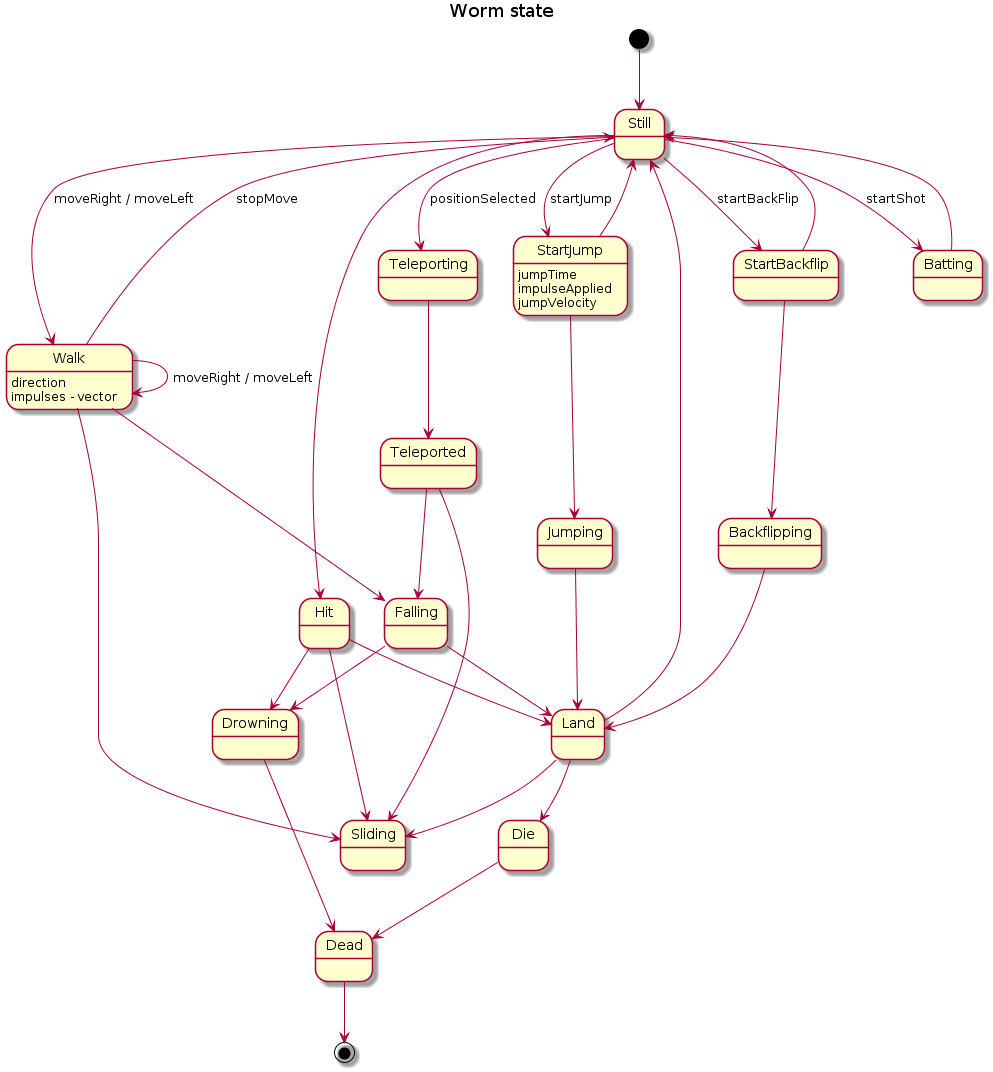
\includegraphics[scale=0.5]{ServerStates.png}
	\caption{Diagrama de estados de los estados posibles del jugador.}
	\label{im:serverState}
\end{sidewaysfigure}

\begin{sidewaysfigure}[!ht]
	\centering
	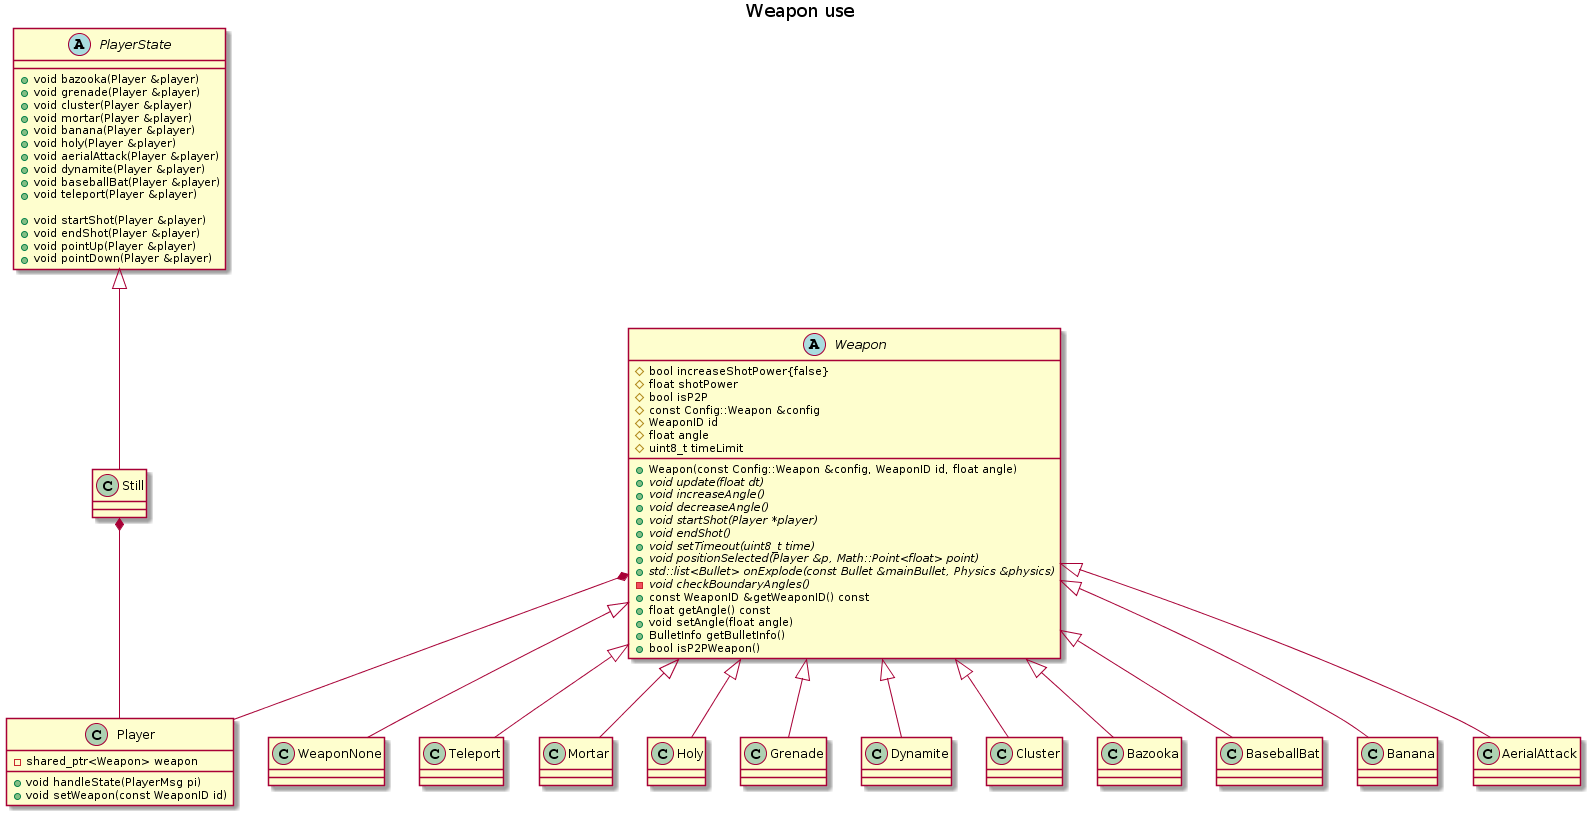
\includegraphics[scale=0.4]{ServerWeapons.png}
	\caption{Diagrama de clase que muestra el uso de las armas.}
	\label{im:serverWeapons}
\end{sidewaysfigure}